\documentclass{article}
\author{}

\usepackage{graphicx}
\usepackage{wrapfig}
\usepackage{enumerate}
\usepackage{hyperref}
\usepackage{float}
\usepackage[margin = 2.25cm]{geometry}
\usepackage[table]{xcolor}
\usepackage{fancyhdr}
\hypersetup{
  colorlinks = true,
  urlcolor = blue
}
\setlength\parindent{0pt}
\pagestyle{fancy}
\fancyhf{}
\rhead{College of Engineering, Construction and Living Sciences\\Bachelor of Information Technology}
\lfoot{Practical 18 React 3: State \& Lifecycle Methods \\Version 1, 2020}
\rfoot{\thepage}

\begin{document}

\begin{figure}
	\centering
	
\includegraphics[width=50mm]{./img/logo.png}
\end{figure}

\title{College of Engineering, Construction and Living Sciences\\Bachelor of Information Technology\\IN608: Intermediate Application Development Concepts\\Level 6, Credits 15\\\textbf{Practical 18 React 3: State \& Lifecycle Methods}} 
\date{}
\maketitle

\textbf{Due Date:} 28/09/2020 at 5pm \\

In this practical, you will complete a series of tasks covering today's lecture. This practical is worth 1\% of the final mark for the IN608: Intermediate Application Development Concepts course. \\

Before you start, in your practicals repository, create a new branch called \textbf{18-practical}.

\section*{Task} 
Create a React app called \texttt{practical18state}. \texttt{cd} to \texttt{practical18state} \& install the following packages:
\begin{itemize}
  \item Axios - \texttt{npm i axios}
  \item Bootstrap - \texttt{npm i bootstrap}
  \item He - \texttt{npm i he}
  \item React spinners - \texttt{npm i react-spinners}
  \item Reactstrap - \texttt{npm i reactstrap}
\end{itemize}

Optionally, you can install all of them at once, i.e., \texttt{npm i axios bootstrap he react-spinners reactstrap}. \\

Create a directory called \texttt{components}. Move \texttt{App.js} into \texttt{components}. Create a file called \texttt{OpenTDB.js}. In \texttt{OpenTDB.js}, create a class called \texttt{OpenTDB} which extends \texttt{React.Component}. In \texttt{OpenTDB}, declare the following constructor:
\begin{verbatim}
  constructor(props) {
    super(props)
    this.state = {
      error: null,
      isLoaded: false,
      data: [],
    }
  }
\end{verbatim}

Below the \texttt{constructor}, declare the following lifecycle method:
\begin{verbatim}
  componentDidMount() {
    axios.get('https://opentdb.com/api.php?amount=5&type=boolean').then(
      (response) => {
        this.setState({
          isLoaded: true,
          data: response.data.results,
        })
      },
      (error) => {
        this.setState({
          isLoaded: true,
          error: error,
        })
      }
    )
  }
\end{verbatim}

\subsection*{What is happening?} 
You are using a promise based HTTP package called \texttt{axios} to request data from an API endpoint using the \texttt{GET} HTTP method. \texttt{then()} method is called \& returns a \texttt{Promise}. It takes up to two arguments: callback functions for the success and failure cases of the \texttt{Promise}. In our case, if success, set the state of \texttt{isLoaded} to \texttt{true} \& \texttt{data} to the response contents from the API request. If failure, set the state of \texttt{isLoaded} to \texttt{true} \& \texttt{error} to error message. \\

In \texttt{render()}, if there is an error display the \texttt{error} state's message. If \texttt{isLoaded} is \texttt{false}, display a loading spinner using \texttt{react-spinners}. If \texttt{isLoaded} is true, return a \texttt{reactstrap} table containing the \texttt{data}. To use \texttt{reactstrap}, you must declare the following in \texttt{index.js}:

\begin{verbatim}
  import 'bootstrap/dist/css/bootstrap.min.css'
\end{verbatim}

This is just a reference to a minified \texttt{CSS} file in the \texttt{bootstrap} package. You will notice some questions contain HTML entities. Encoding works slightly different in React \& you need to use \texttt{he} to do this. If there is no \texttt{data}, display the message \texttt{No data available.} in the \texttt{reactstrap} table. This message should span four table columns. \\

In \texttt{App.js}, call the \texttt{OpenTDB} component. Your \texttt{App.js} file should look like the following:

\begin{verbatim}
  import React from 'react'
  import OpenTDB from './OpenTDB'

  class App extends React.Component {
    render() {
      return (
        <div className='container'>
          <OpenTDB />
        </div>
      )
    }
  }

  export default App
\end{verbatim}

\subsection*{Expected Output} 
Run the command \texttt{npm start} then navigate to \href{http://localhost:3000/}{http://localhost:3000/} \\

\begin{figure}[H]
  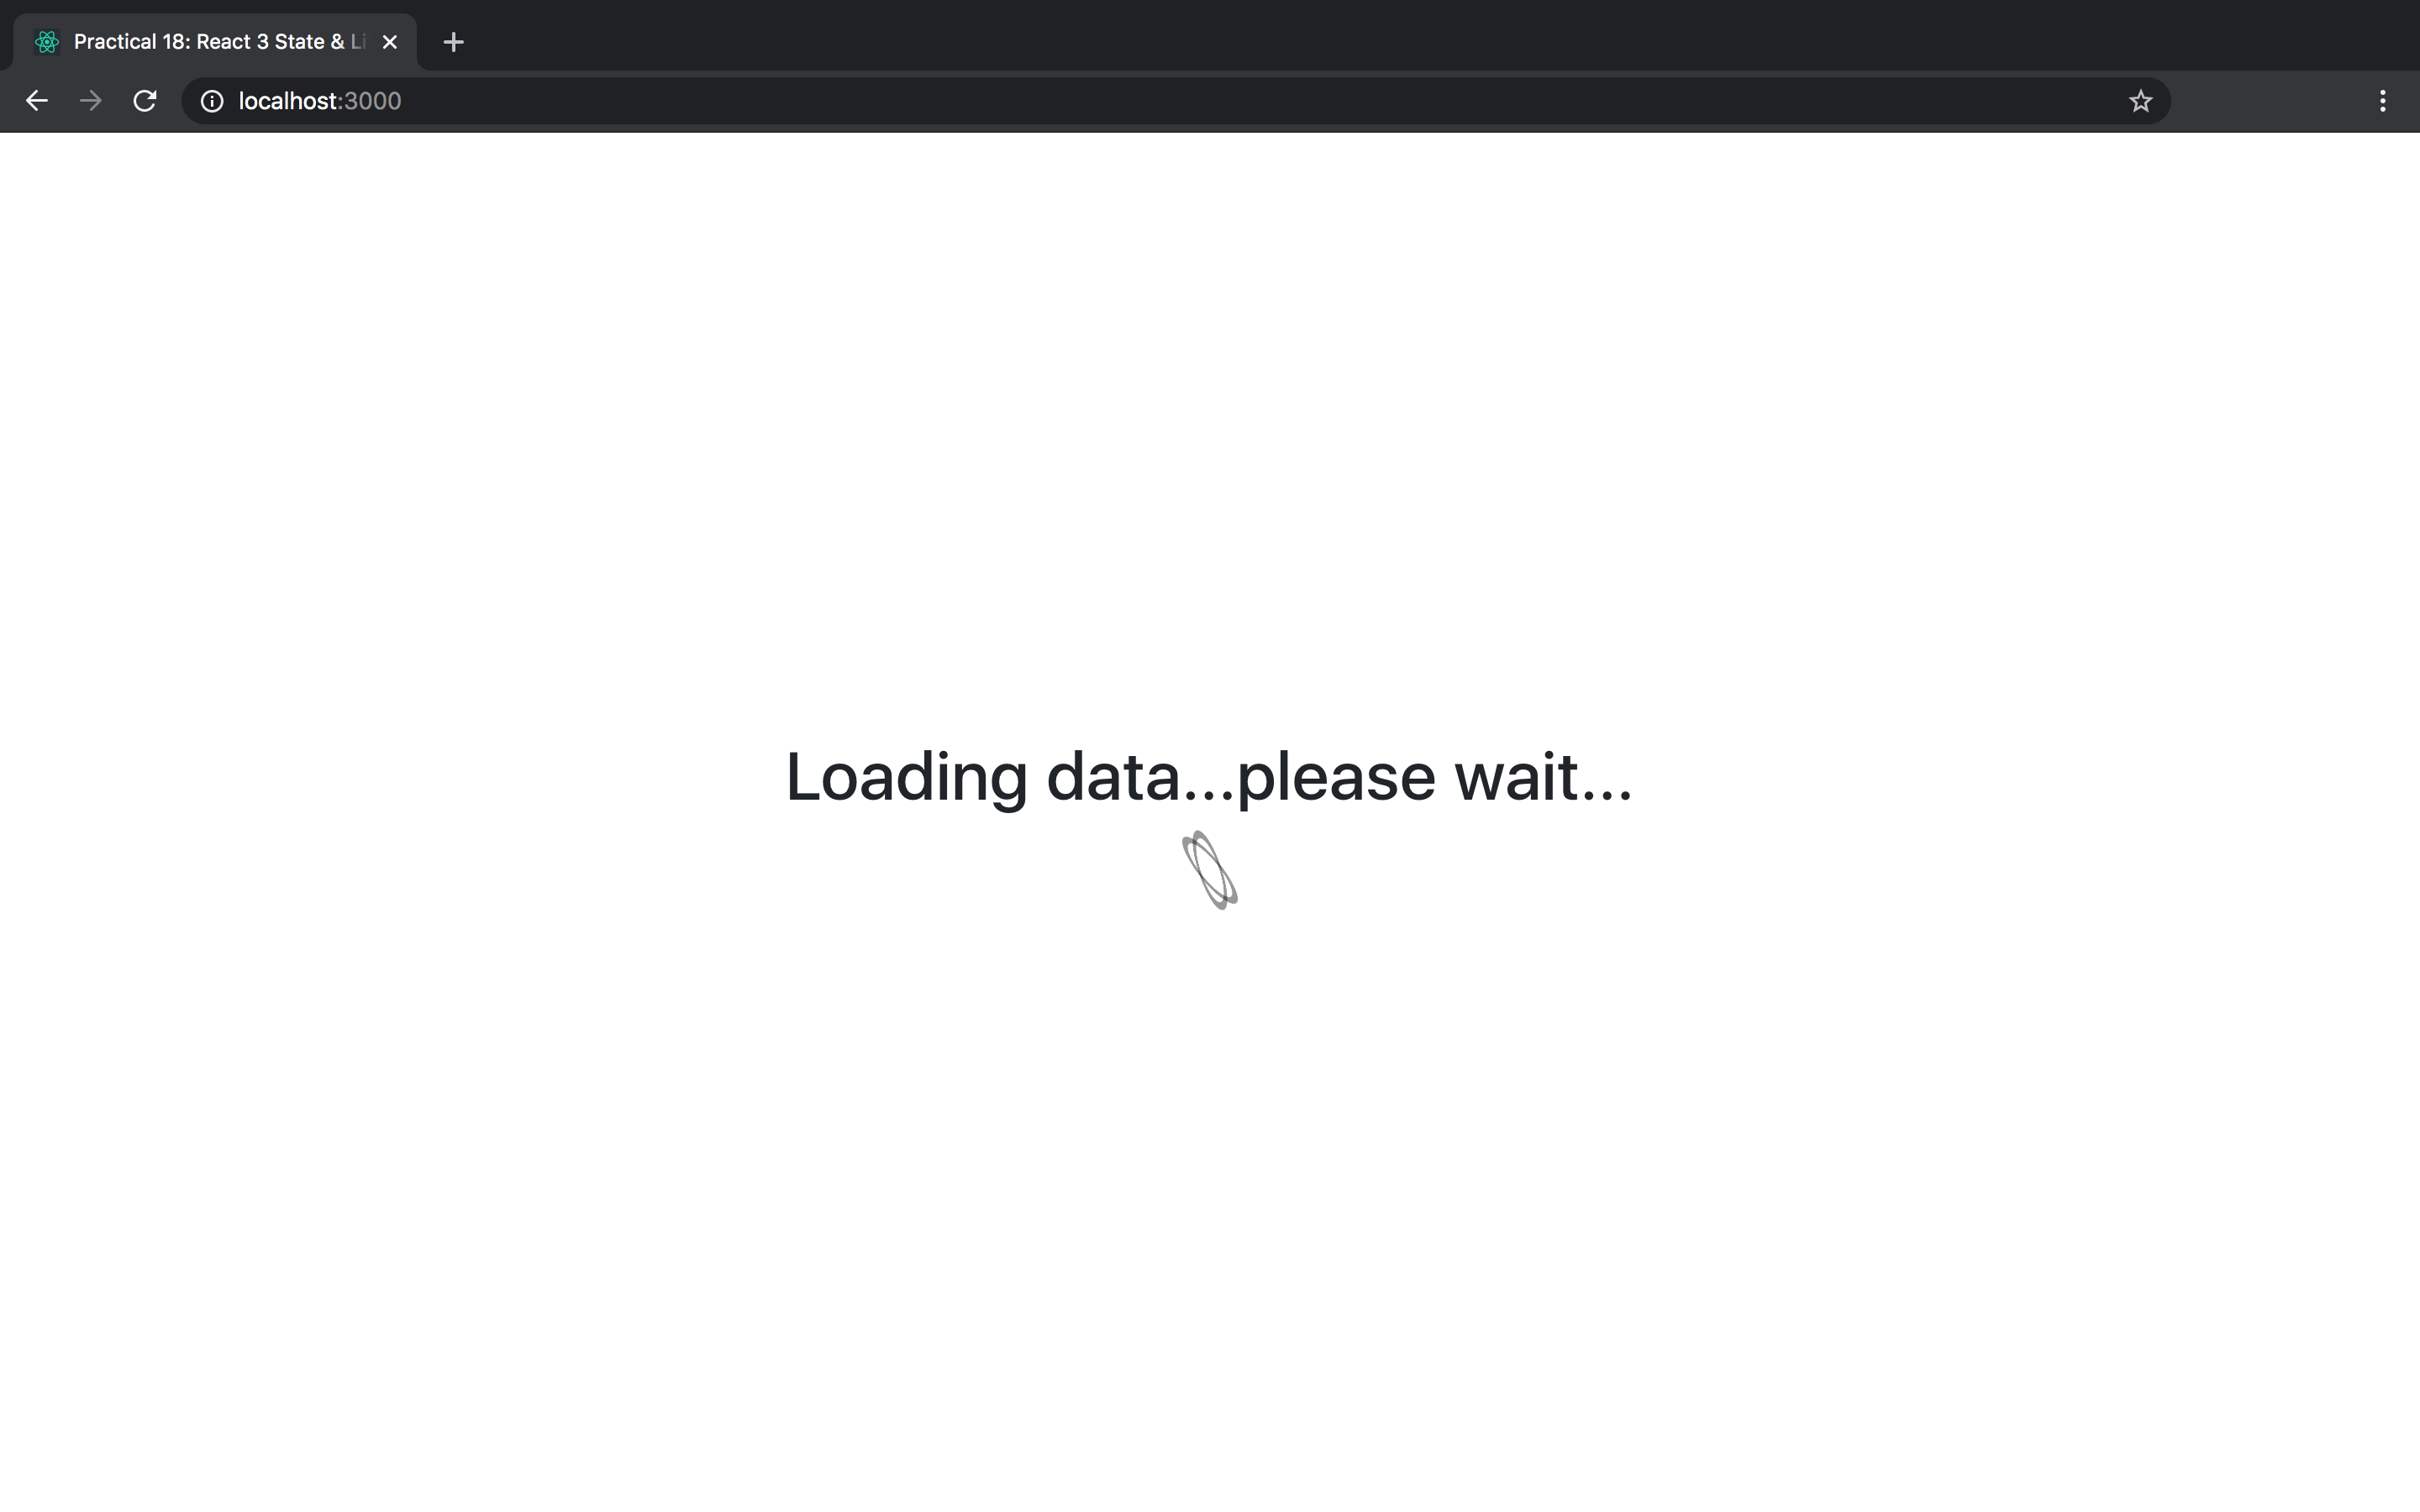
\includegraphics[width=175mm, height=105mm]{./img/18-expected-opentdb-1.png}
  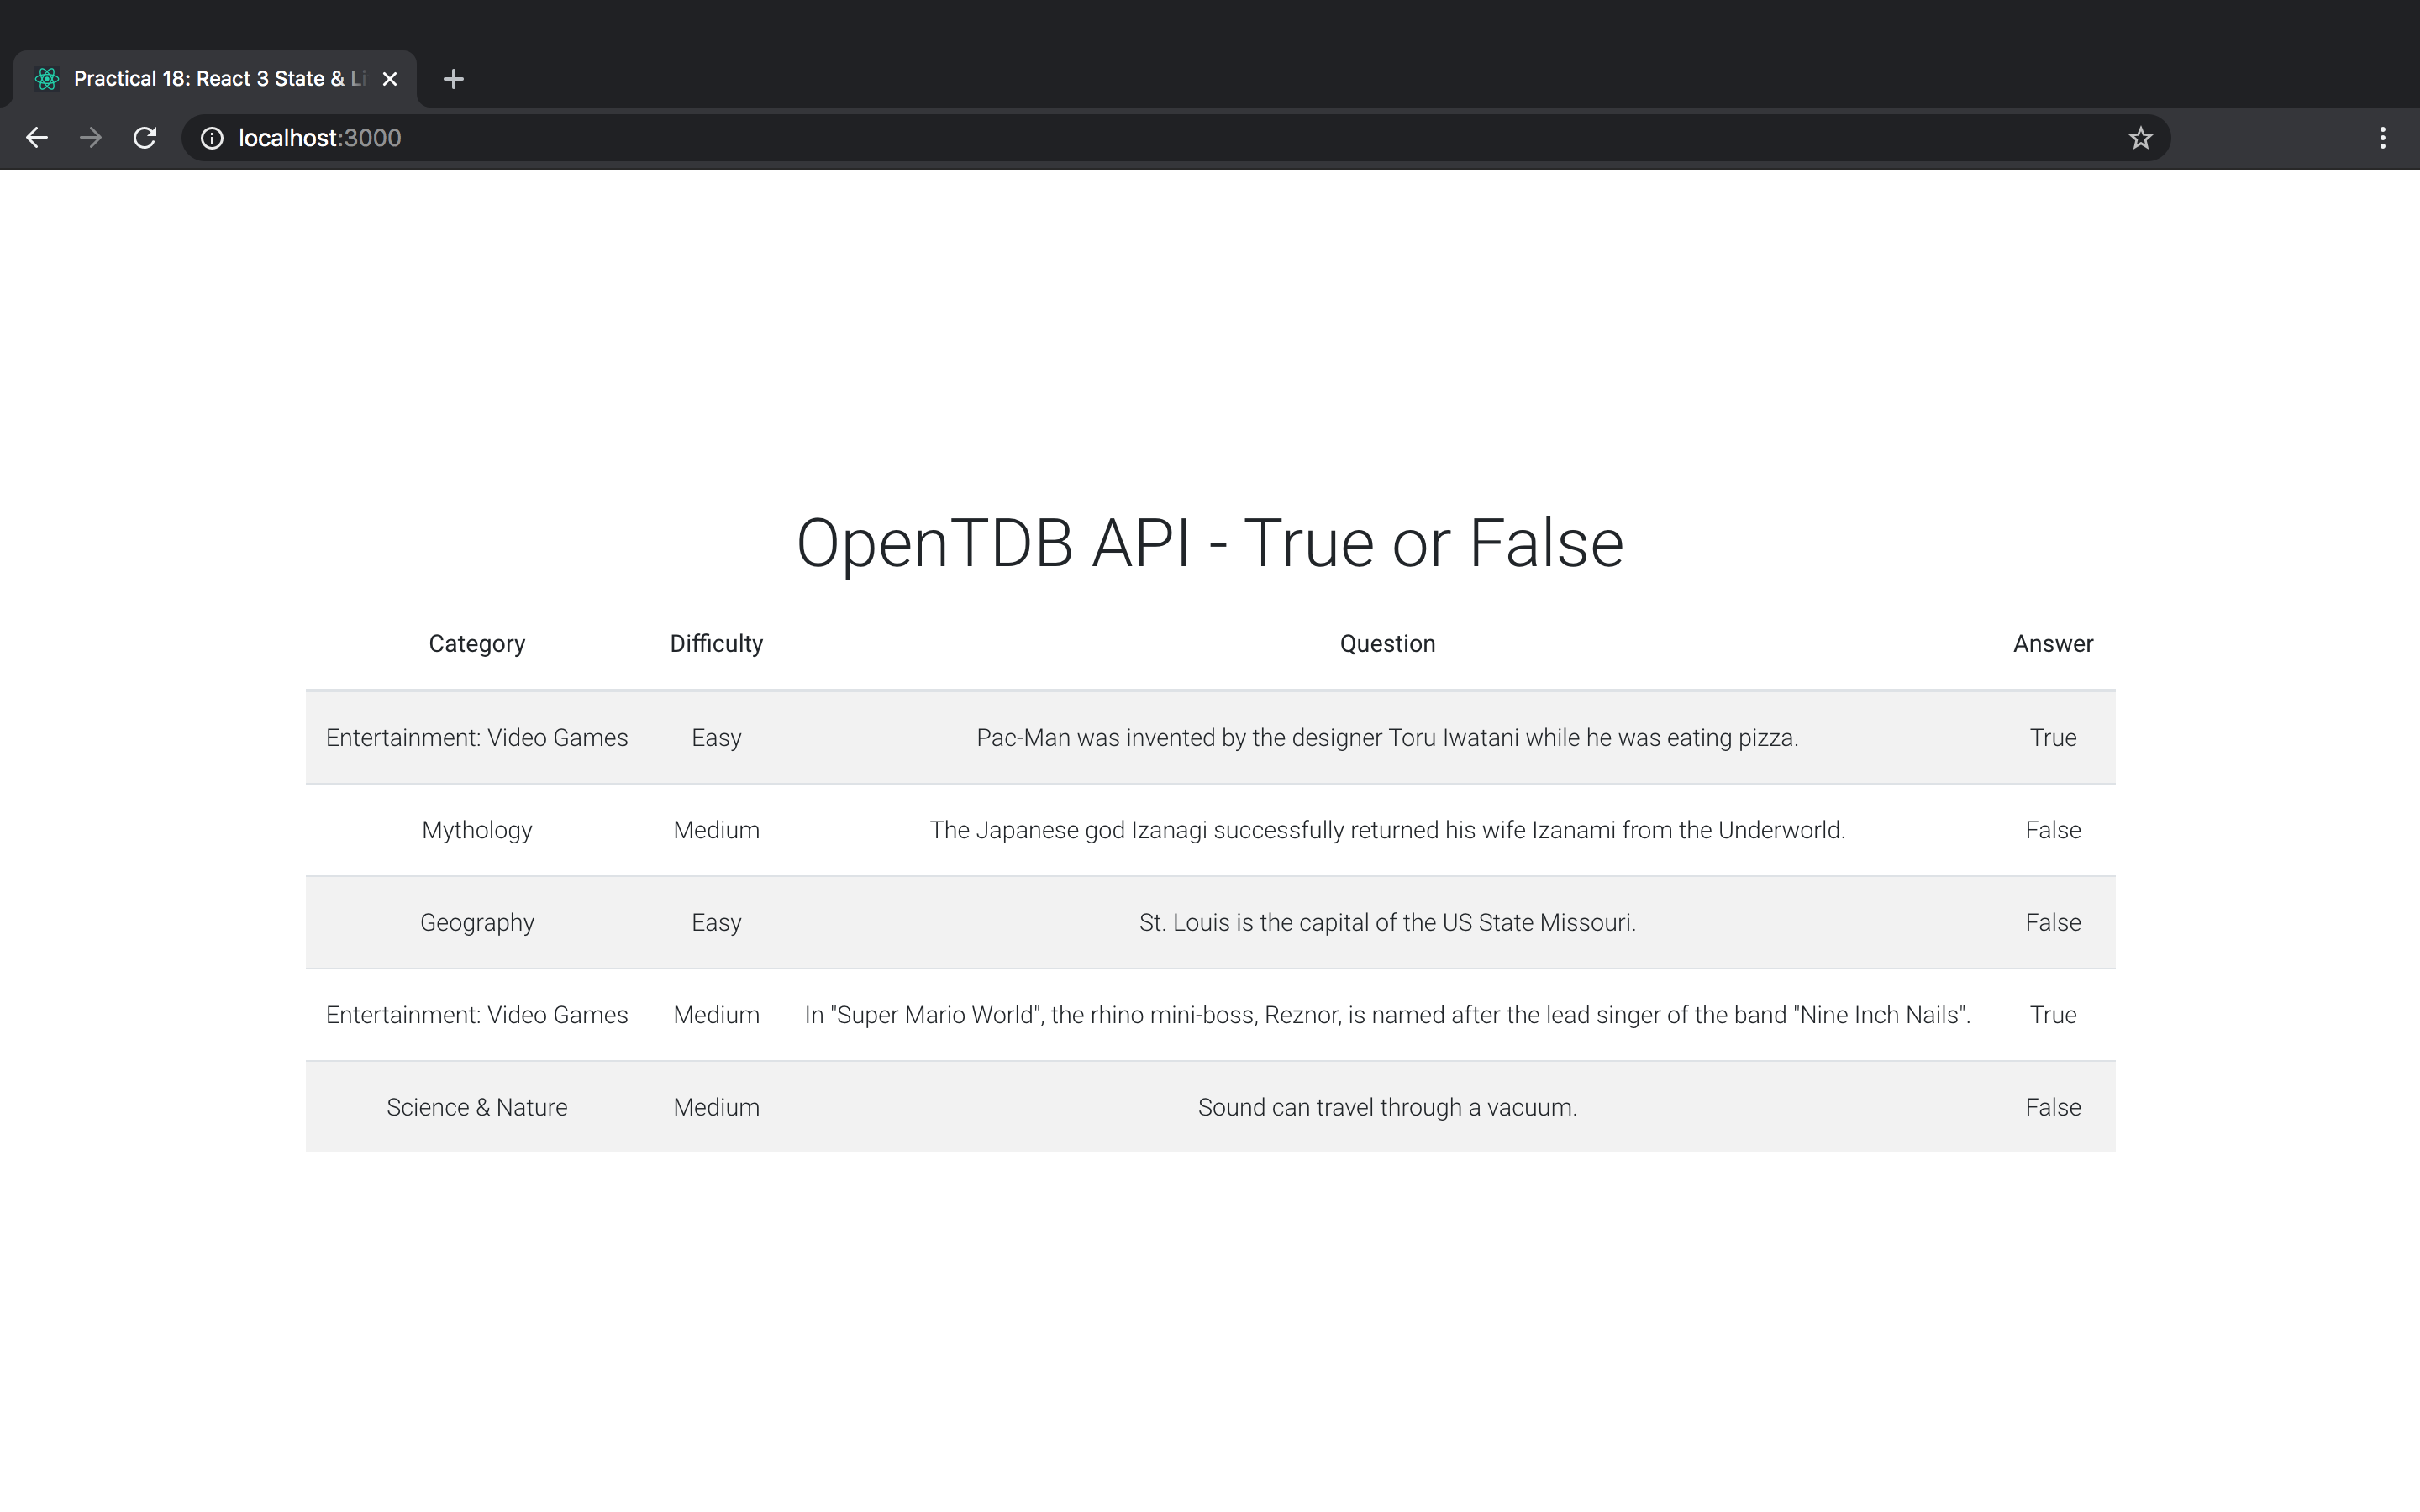
\includegraphics[width=175mm, height=105mm]{./img/18-expected-opentdb-2.png}
\end{figure}

\begin{figure}[H]
  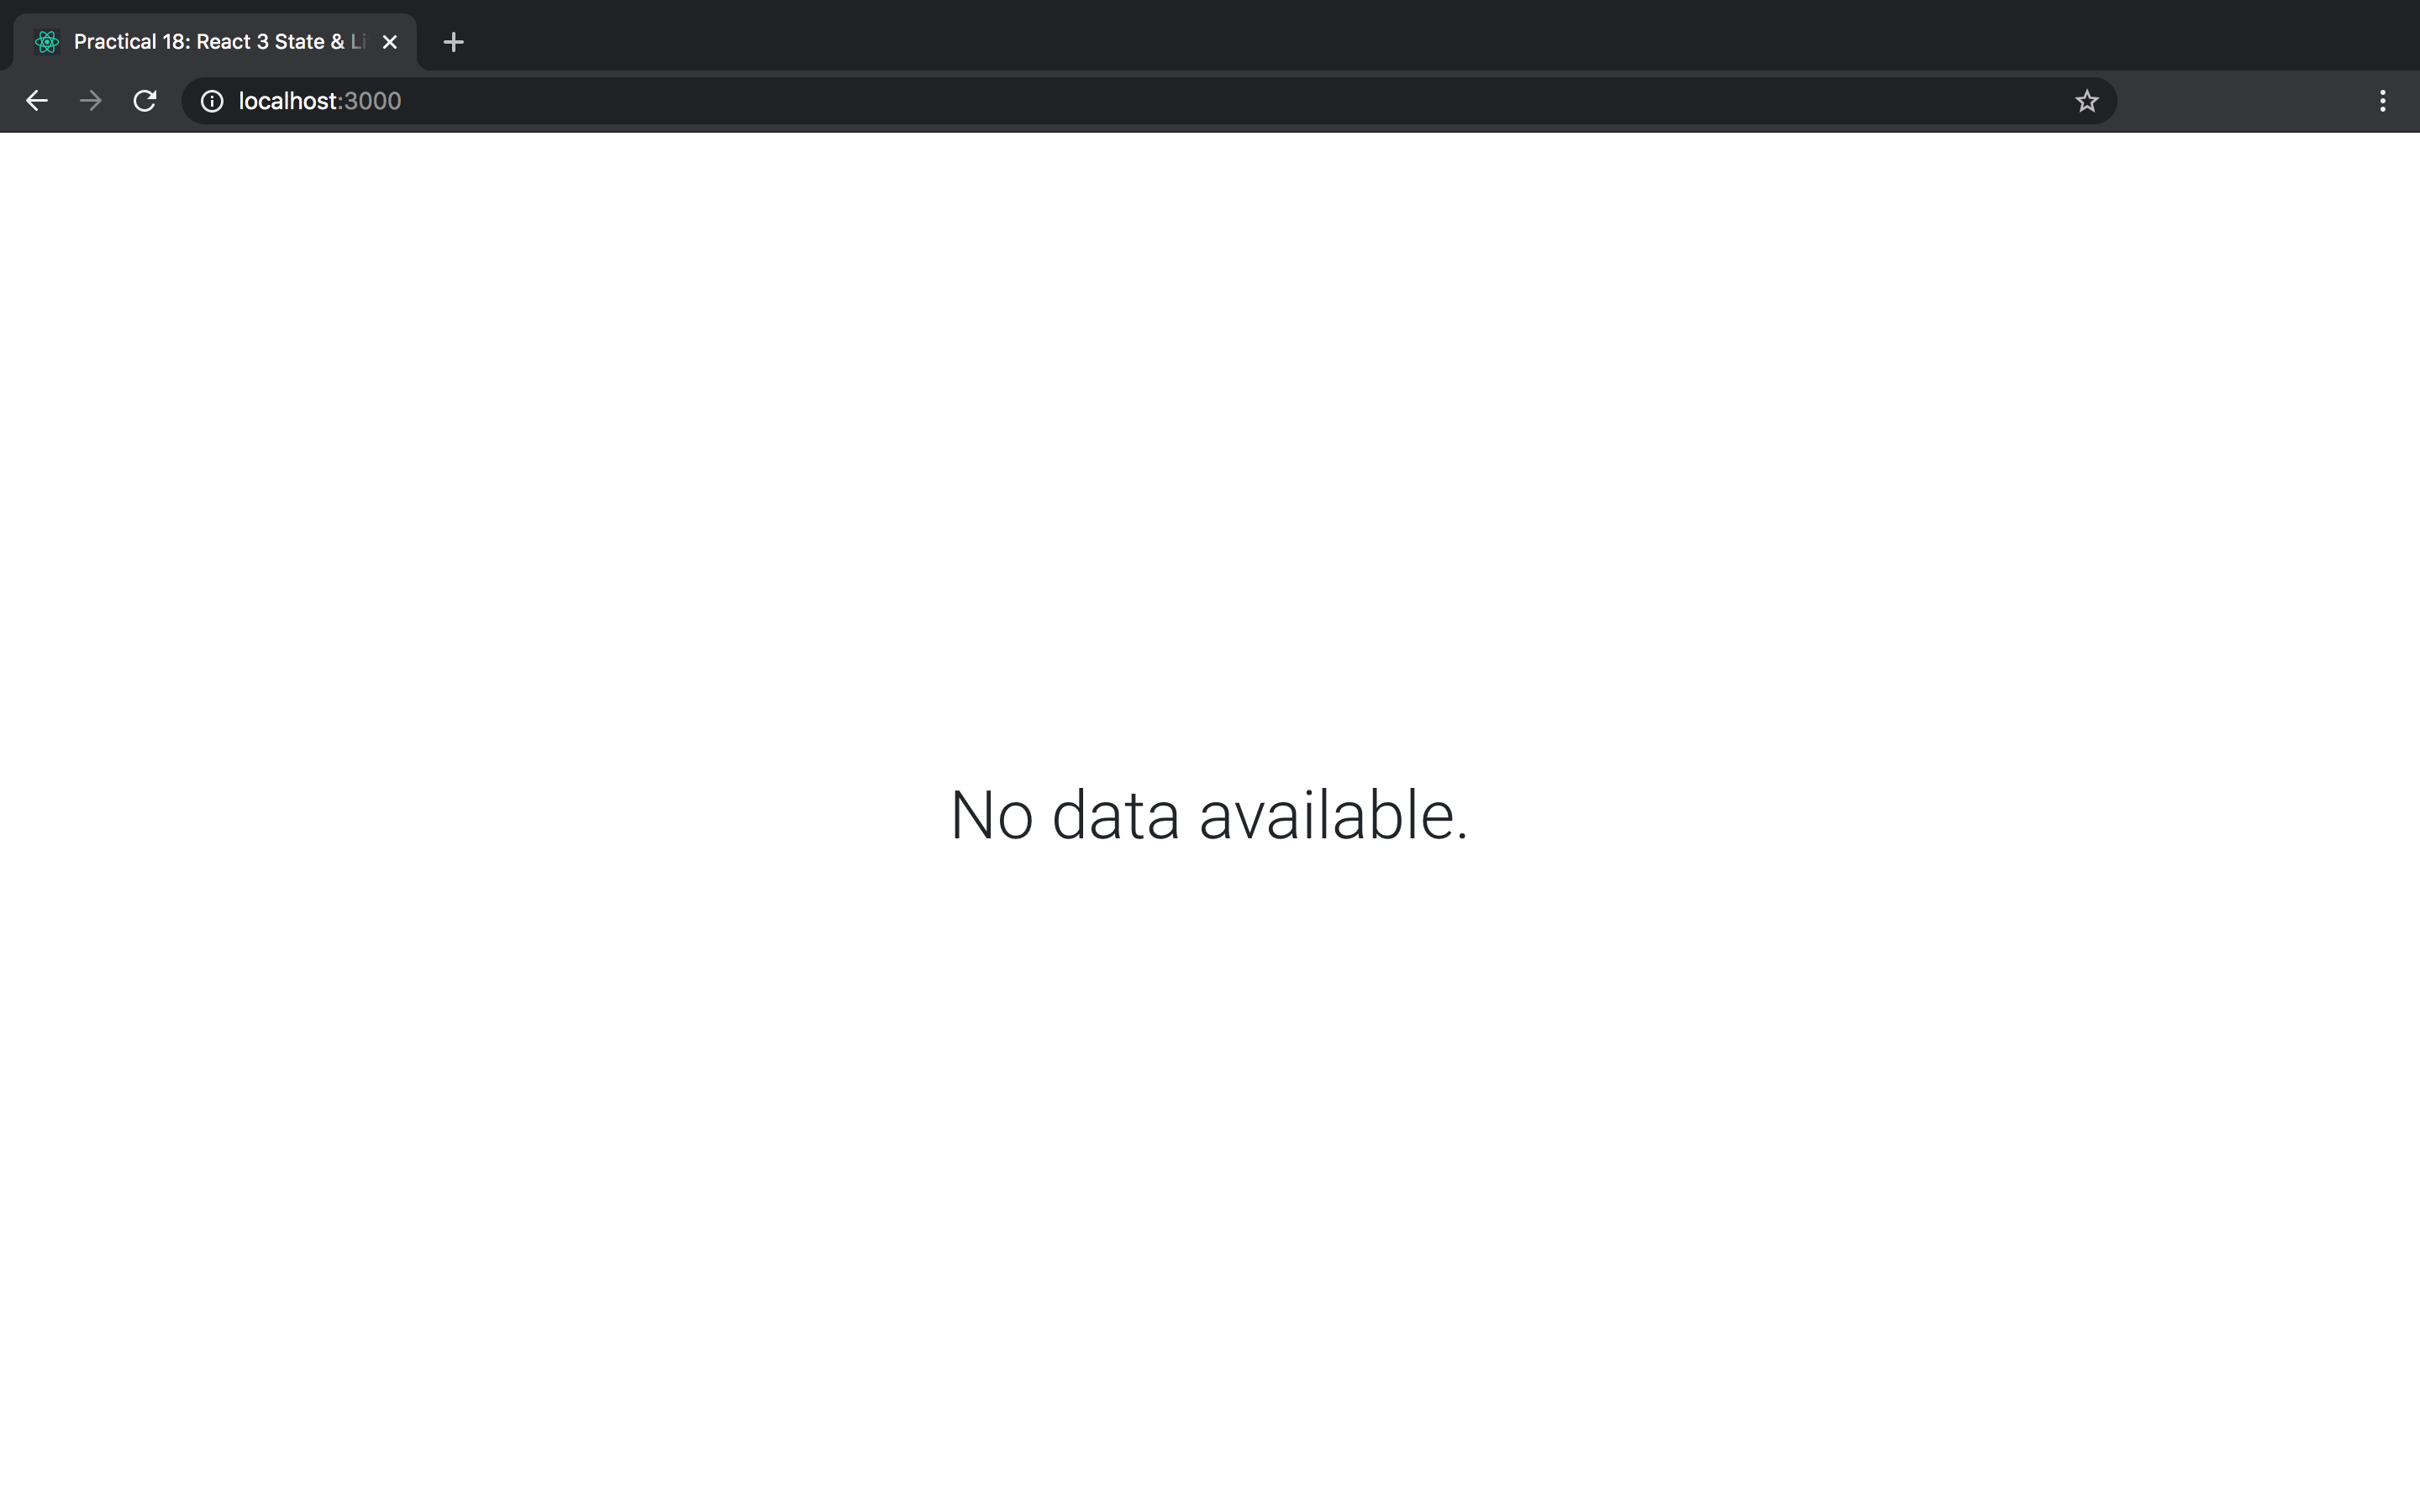
\includegraphics[width=175mm, height=105mm]{./img/18-expected-opentdb-3.png}
  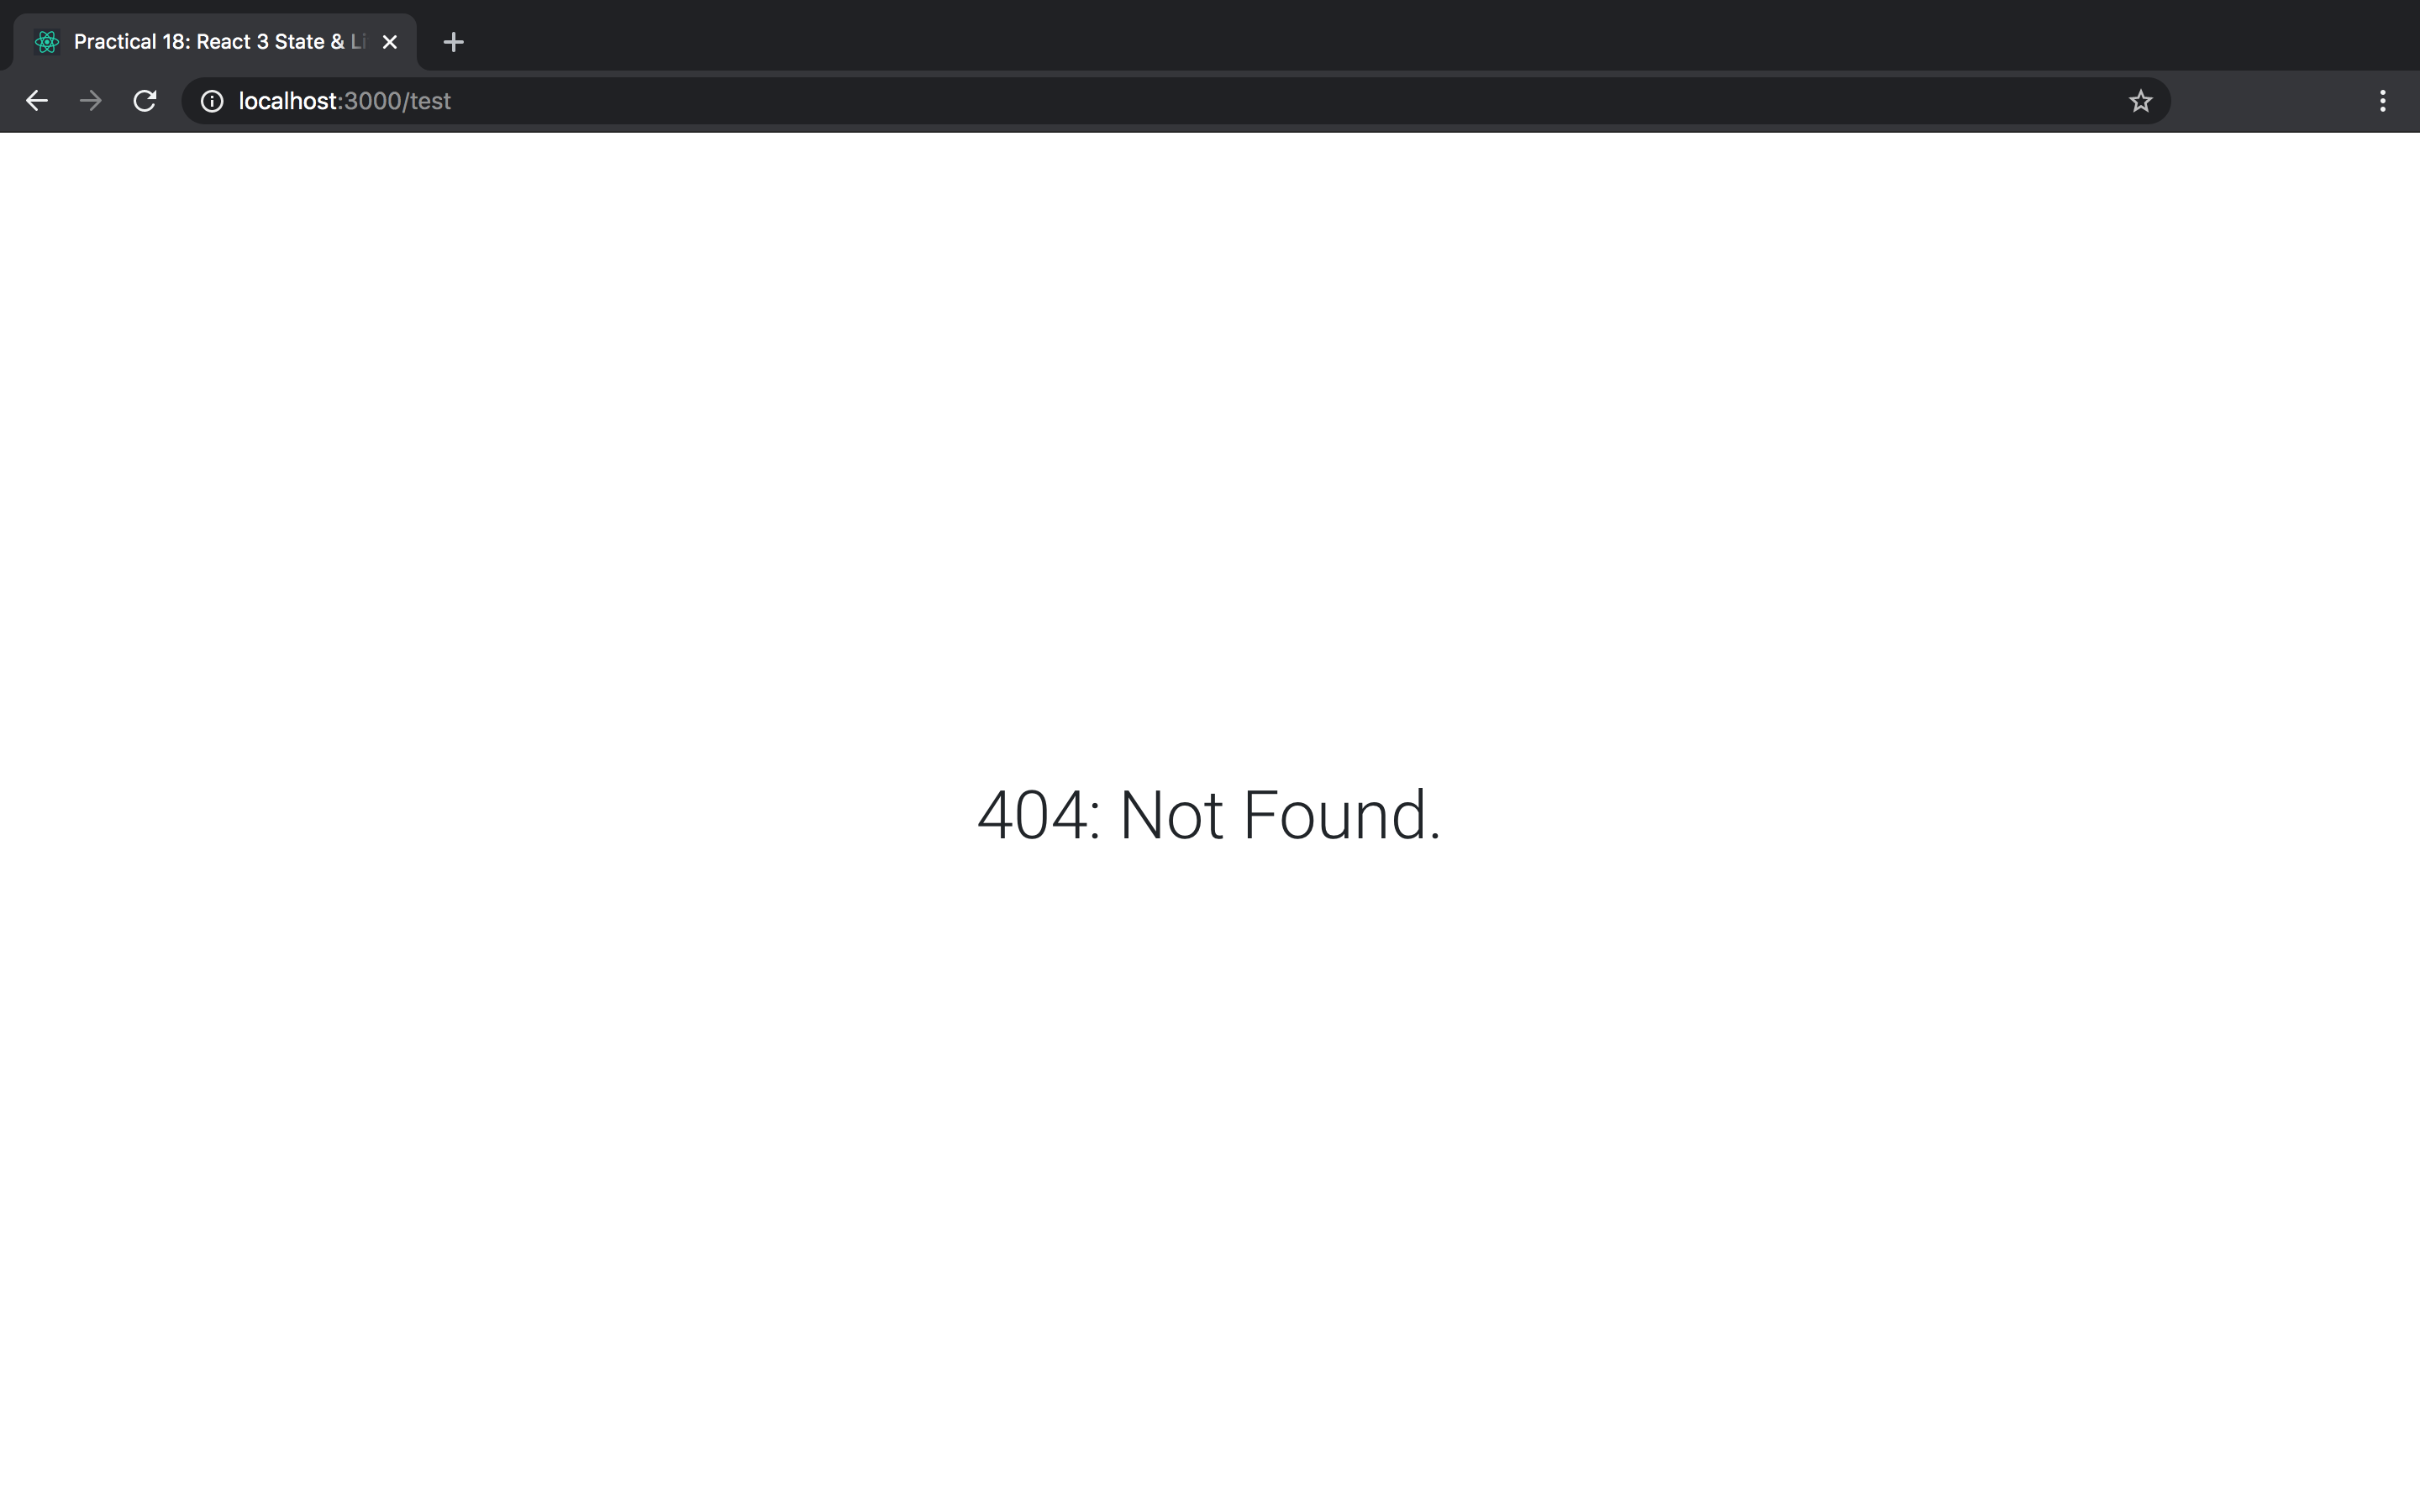
\includegraphics[width=175mm, height=105mm]{./img/18-expected-opentdb-4.png}
\end{figure}

\textbf{Deployment link:} \href{https://int-app-dev-practical-18.herokuapp.com/}{https://int-app-dev-practical-18.herokuapp.com/} 

\subsection*{Resources} 
\begin{itemize}
  \item \href{https://opentdb.com/}{OpenTDB API}
  \item \href{https://www.npmjs.com/package/axios/}{Axios}
  \item \href{https://getbootstrap.com/}{Bootstrap}
  \item \href{https://www.npmjs.com/package/he/}{He}
  \item \href{https://www.npmjs.com/package/react-spinners/}{React spinners}
  \item \href{https://www.npmjs.com/package/reactstrap/}{Reactstrap}
\end{itemize}
 
\end{document}